\documentclass[conference]{IEEEtran}

\usepackage[T1]{fontenc}
\usepackage{cite}
\usepackage{amsmath,amssymb,amsfonts}
\usepackage{graphicx}
\usepackage{textcomp}
\usepackage{xcolor}
\usepackage{booktabs}
\usepackage{multirow}
\usepackage{url}
\usepackage{microtype}
\usepackage{subcaption}

\def\BibTeX{{\rm B\kern-.05em{\sc i\kern-.025em b}\kern-.08em
    T\kern-.1667em\lower.7ex\hbox{E}\kern-.125emX}}

\begin{document}

\title{A Framework for Scientific Article Classification and Recommendation Using NLP and Machine Learning}

\author{
\IEEEauthorblockN{Abdullah Al Mahmud}
\IEEEauthorblockA{
Department of Computer Science \& Engineering\\
BRAC University\\
Dhaka, Bangladesh\\
\texttt{abdullah.al.mahmud@g.bracu.ac.bd}
}
}

\maketitle

% ─────────────────────────────────────────────────────────────
%  ABSTRACT
% ─────────────────────────────────────────────────────────────
\begin{abstract}
This paper presents a machine learning pipeline that classifies
scientific articles and recommends related papers using the arXiv
dataset.  The classification part fine-tunes a DistilBERT model
to predict one of 20 arXiv subject categories from a paper's title.
The recommendation part encodes titles into dense vectors using the
all-MiniLM-L6-v2 sentence-transformer and retrieves similar papers
via cosine similarity.  We build a balanced dataset of 37,855 papers
across 20 categories after preprocessing.  The classifier reaches
67.65\% test accuracy and a weighted F1-score of 0.67.  Strong
per-class F1-scores are seen for \texttt{math.CO} (0.86),
\texttt{cs.CL} (0.84), and \texttt{cs.CV} (0.83).  Both components
are combined into a single pipeline that takes a text query and
returns category predictions alongside paper recommendations.
\end{abstract}

\begin{IEEEkeywords}
Article classification, scientific recommendation, DistilBERT,
sentence transformers, natural language processing, arXiv,
cosine similarity, transfer learning
\end{IEEEkeywords}

% ─────────────────────────────────────────────────────────────
%  I. INTRODUCTION
% ─────────────────────────────────────────────────────────────
\section{Introduction}

There are now over 50 million scholarly articles published across
various repositories, and new papers are added every day.  For a
researcher, finding the right paper can take a lot of time,
especially when entering a new area.  Simple keyword search often
misses papers that are relevant but use different words.

Pretrained language models have made it much easier to build systems
that understand the meaning of text.  BERT \cite{devlin2018bert} in
particular showed that a model trained on large amounts of text can
be fine-tuned for many downstream tasks with strong results.
Sentence-transformer models \cite{reimers2019sentence} take this
further by producing compact embeddings that can be compared
efficiently across thousands of documents.

In this work, we build a two-part system using arXiv paper titles.
The first part classifies a title into one of 20 subject categories.
The second part recommends similar papers using semantic similarity.
The goal is to help researchers quickly find where a paper belongs
and what related work exists.

Our main contributions are:

\begin{itemize}
  \item Fine-tuning DistilBERT on arXiv paper titles for 20-class
    classification, reaching 67.65\% test accuracy from title text alone.
  \item Building a semantic similarity index using the all-MiniLM-L6-v2
    sentence-transformer for content-based paper recommendation.
  \item Curating a cleaned and balanced arXiv dataset of 37,855 papers
    across 20 primary subject categories.
  \item Integrating both components into a unified inference pipeline
    that takes a single text query and returns both predictions and
    recommendations.
\end{itemize}

The rest of the paper covers related work, methodology, results,
limitations, future directions, and a conclusion.

% ─────────────────────────────────────────────────────────────
%  II. RELATED WORK
% ─────────────────────────────────────────────────────────────
\section{Related Work}
\label{sec:related}

\subsection{Text Classification}

Early text classification methods used word frequency features like
TF-IDF with classical classifiers such as Naive Bayes, Support Vector
Machines, and Random Forests.  These methods worked reasonably well
but depended heavily on feature engineering.

The introduction of BERT \cite{devlin2018bert} changed the field
significantly.  By pretraining on large corpora and fine-tuning on
specific tasks, BERT-based models achieved strong results across many
classification benchmarks.  Lightweight variants like DistilBERT
kept most of this performance while being faster and cheaper to run.

\subsection{Scientific Recommendation Systems}

Recommending academic papers is a well-studied problem.
Beel~et~al.~\cite{beel2016paper} surveyed many approaches including
collaborative filtering and content-based filtering, and noted that
purely similarity-based methods struggle when user history is limited.

Sentence-level embeddings have become a popular solution for
content-based recommendation.  Reimers and
Gurevych~\cite{reimers2019sentence} introduced Sentence-BERT, which
produces fixed-length embeddings suitable for efficient similarity
search.  The Universal Sentence Encoder~\cite{cer2018universal}
offers similar capabilities through multi-task training, generalizing
well across retrieval and classification tasks.

\subsection{Topic Modeling and Semantic Similarity}

Topic models like Latent Dirichlet Allocation
\cite{blei2003latent} have been used to explore the structure of
large document collections.  They give a high-level view of what
themes are present in a corpus, complementing the finer-grained
per-document predictions that classification models produce.
Cosine similarity over dense embeddings has largely replaced
topic models for retrieval tasks, as it is faster and captures
richer semantic information.

% ─────────────────────────────────────────────────────────────
%  III. METHODOLOGY
% ─────────────────────────────────────────────────────────────
\section{Methodology}
\label{sec:method}

\subsection{Dataset Collection and Description}

We use the publicly available arXiv metadata snapshot, which
contains paper identifiers, titles, abstracts, and subject
category tags.  We identify the 20 most frequent primary category
tags and keep papers that belong to at least one of them.  Each
paper is then assigned its first listed category as the primary
label, and up to 2,500 papers are sampled per category, giving
47,500 records before cleaning.

After removing papers with missing titles and those whose primary
category falls outside the top-20 set, the final corpus contains
\textbf{37,855} papers.  These span astrophysics, condensed matter
physics, computer science, mathematics, high-energy physics, and
statistics subcategories.

Figure~\ref{fig:category_dist} shows the distribution across all
20 categories after preprocessing.

\begin{figure}[htbp]
  \centering
  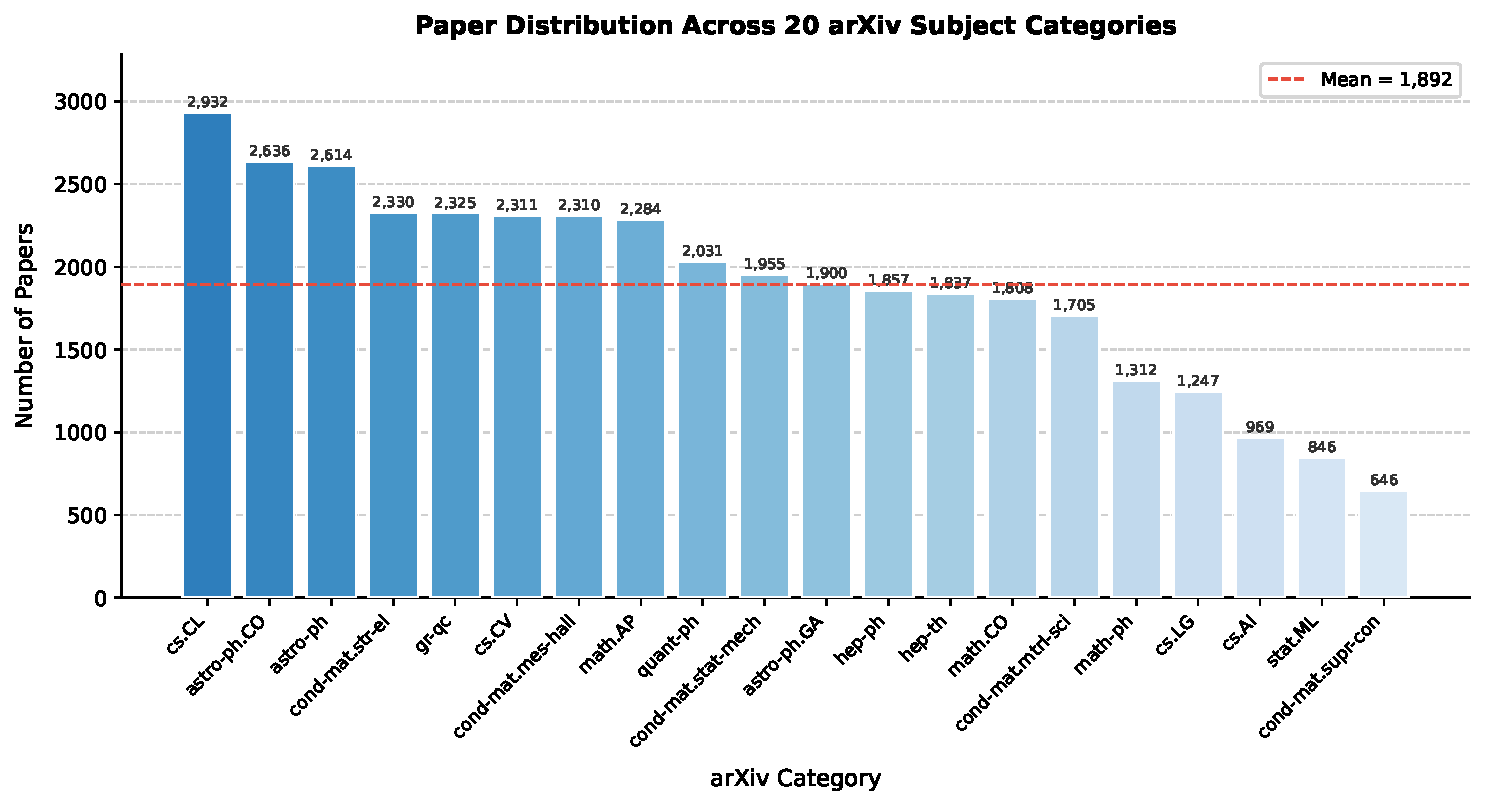
\includegraphics[width=\columnwidth]{figures/fig2_category_distribution.pdf}
  \caption{Distribution of papers across the 20 arXiv subject
    categories after preprocessing, sorted by paper count.}
  \label{fig:category_dist}
\end{figure}

\subsection{Data Preprocessing}

We extract each paper's primary category from its first listed tag.
Papers with blank titles or primary categories outside the top-20
set are removed.  String labels are converted to integer indices
using a \texttt{LabelEncoder}, keeping a consistent mapping
throughout training and inference.

The dataset is split into training (75\%), validation (10\%), and
test (15\%) subsets using stratified sampling, which preserves
class proportions in each split.  This gives roughly 28,391
training, 3,786 validation, and 5,678 test samples.

Figures~\ref{fig:pipeline}, \ref{fig:title_length},
and~\ref{fig:datasplit} show the full pipeline, the title length
distribution, and the dataset split proportions respectively.

\begin{figure}[htbp]
  \centering
  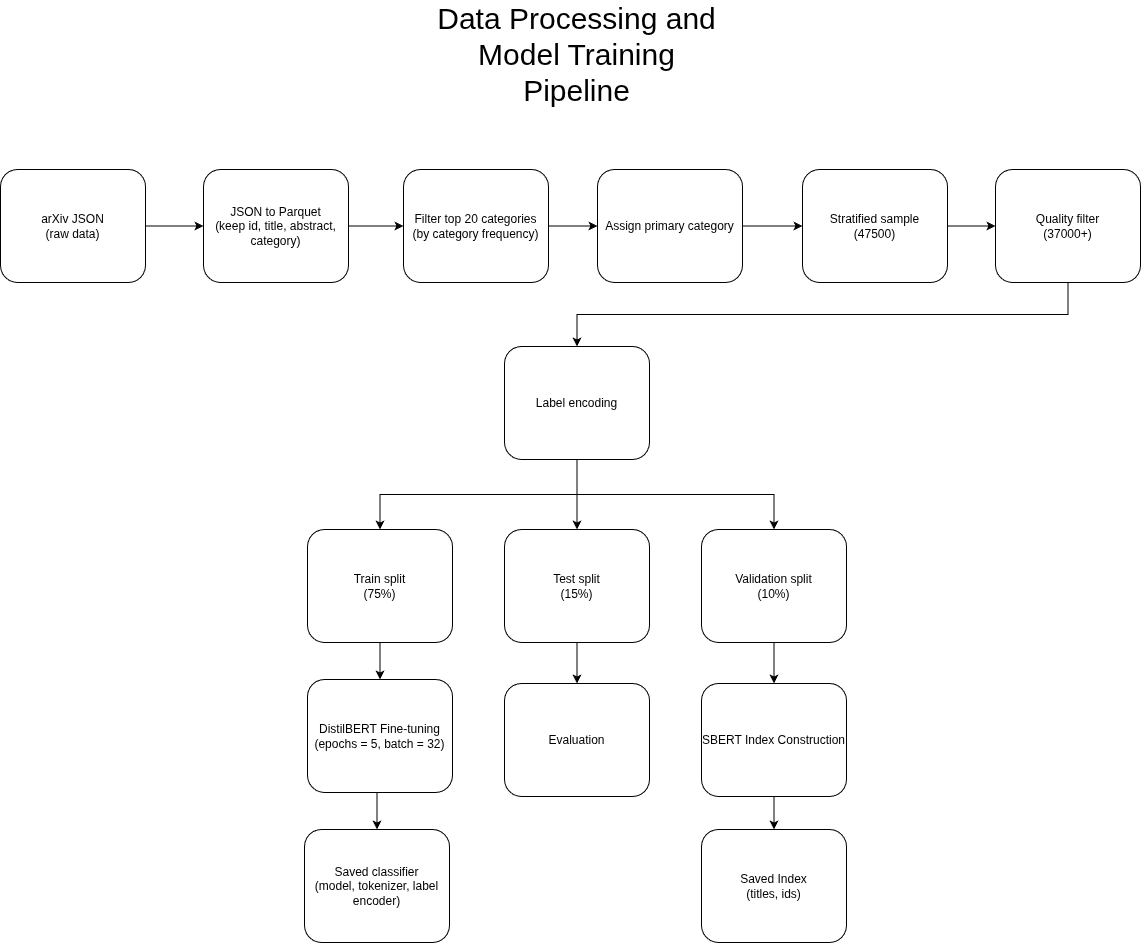
\includegraphics[width=\columnwidth]{figures/data_processing.png}
  \caption{Full data preprocessing and model training pipeline from
    raw arXiv JSON to final inference.}
  \label{fig:pipeline}
\end{figure}

\begin{figure}[htbp]
  \centering
  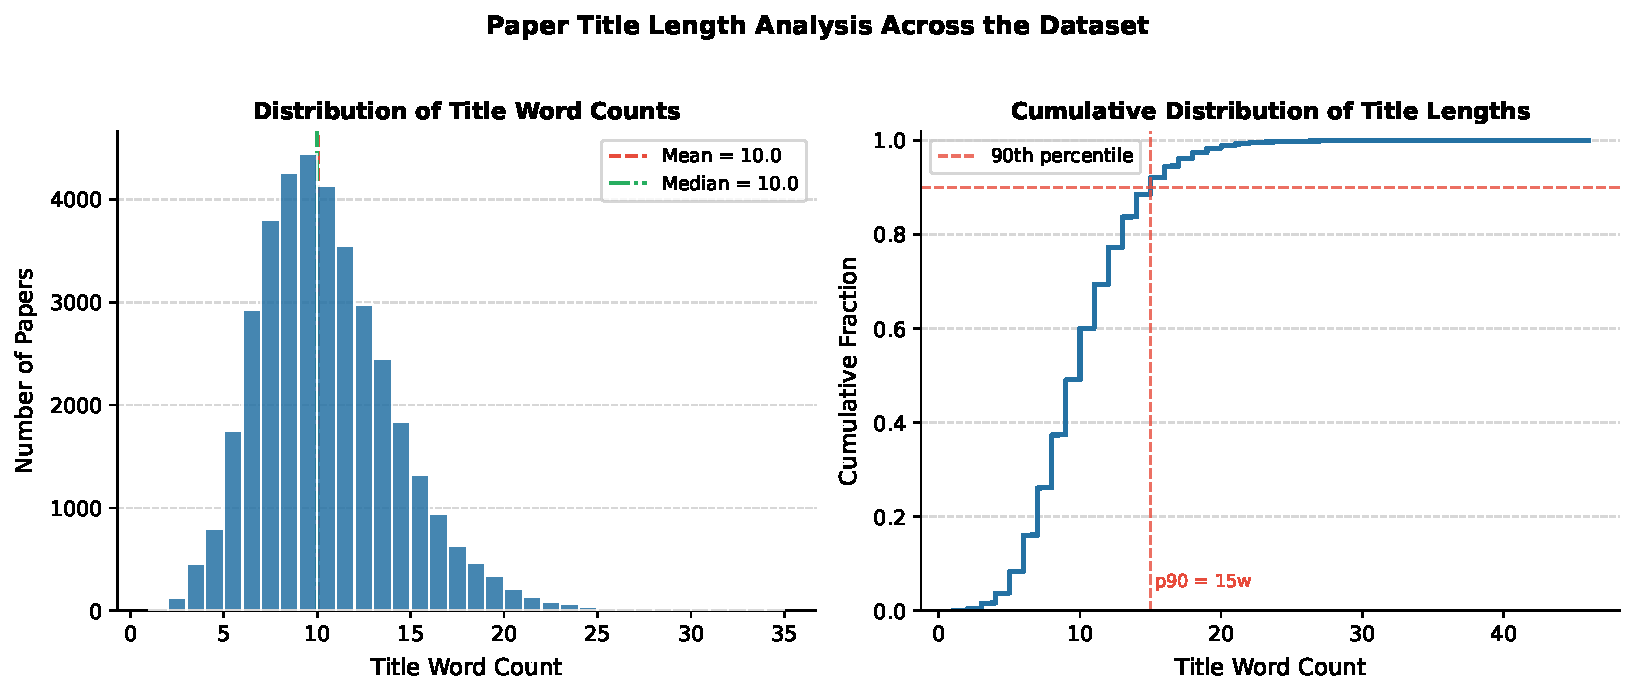
\includegraphics[width=\columnwidth]{figures/fig3_title_length.pdf}
  \caption{Distribution of word counts in paper titles.  Most titles
    are between 5 and 15 words long.}
  \label{fig:title_length}
\end{figure}

\begin{figure}[htbp]
  \centering
  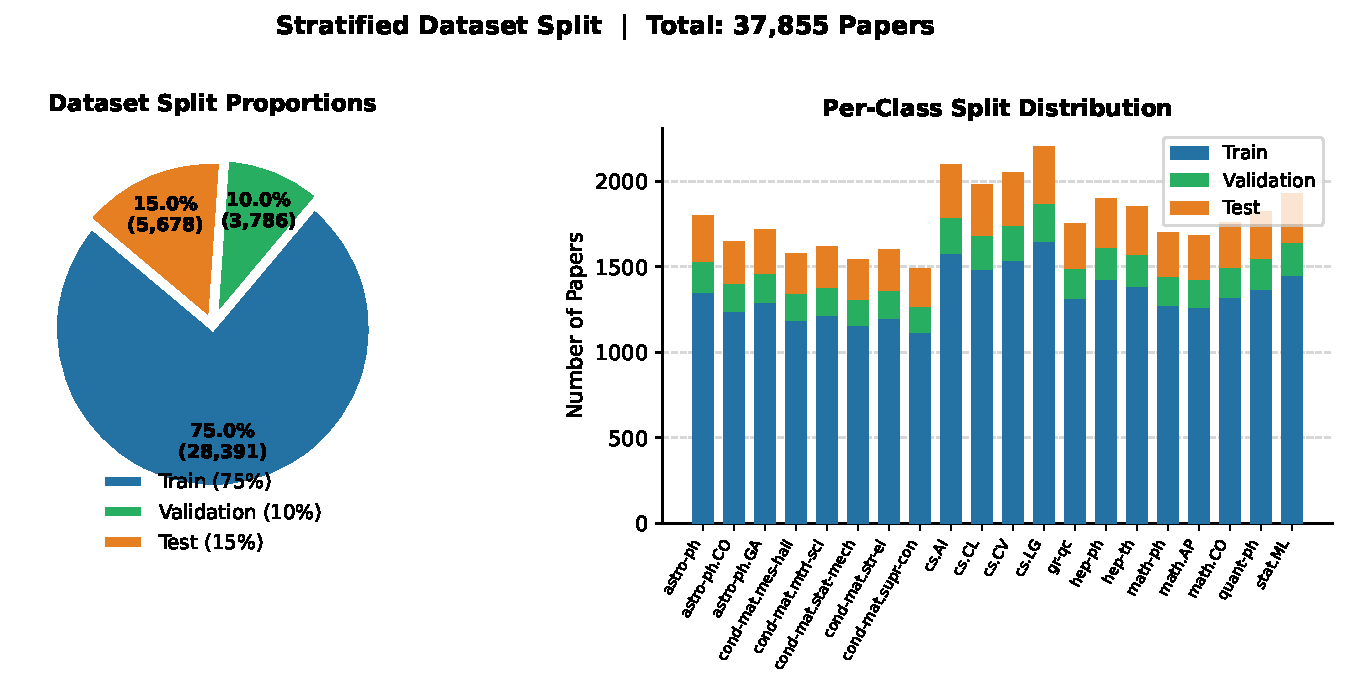
\includegraphics[width=\columnwidth]{figures/fig4_data_split.pdf}
  \caption{Dataset split into training (75\%), validation (10\%),
    and test (15\%) partitions, stratified by class label.}
  \label{fig:datasplit}
\end{figure}

\subsection{Classifier Architecture and Training}

We fine-tune DistilBERT \cite{devlin2018bert}, starting from the
\texttt{distilbert-base-uncased} checkpoint.  A linear head is added
on top that maps the pooled output to a 20-class logit vector.
Titles are tokenized and padded or truncated to 128 tokens, which
is more than enough for most arXiv titles.

We train with the AdamW optimizer at a learning rate of
$2 \times 10^{-5}$, gradient clipping at norm 1.0, and a linear
decay schedule.  Training runs for five epochs with batch size 32,
saving the best checkpoint by validation accuracy.  Training takes
about 15 minutes on an NVIDIA RTX 3060 GPU with 12 GB VRAM.

\subsection{Recommendation System}

The recommender uses the \texttt{all-MiniLM-L6-v2}
sentence-transformer to encode all training titles into
384-dimensional vectors.  These are stored in an index file.
At query time, the user's input is encoded the same way, and
cosine similarity is computed against the full index:

\begin{equation}
  \text{sim}(\mathbf{q}, \mathbf{d})
    = \mathbf{q} \cdot \mathbf{d}
    = \sum_{i=1}^{384} q_i d_i
  \label{eq:cosine}
\end{equation}

The top-$k$ most similar papers are returned.  Since all embeddings
are L2-normalized, the dot product equals cosine similarity.
This brute-force approach works well for corpora of this size
without any extra infrastructure.

\subsection{Unified Inference Pipeline}

At inference time, both the DistilBERT classifier and the
sentence-transformer index are loaded once into memory.
Given a query string, the classifier returns top-$k$ category
predictions with confidence scores, while the recommender returns
the top-$k$ most similar paper titles with similarity scores.
Both outputs are returned together.

Figure~\ref{fig:architecture} shows the overall system design.

\begin{figure}[htbp]
  \centering
  \includegraphics[width=\columnwidth]{figures/system_architecture.png}
  \caption{System architecture.  A query feeds both the DistilBERT
    classifier and the sentence-transformer recommender in parallel,
    returning category predictions and similar papers.}
  \label{fig:architecture}
\end{figure}

% ─────────────────────────────────────────────────────────────
%  IV. RESULTS
% ─────────────────────────────────────────────────────────────
\section{Results}
\label{sec:results}

\subsection{Experimental Setup}

All experiments ran on Ubuntu Linux with an NVIDIA RTX 3060 GPU
(12 GB VRAM), 32 GB RAM, and CUDA 12.4.  The classifier uses
Hugging Face Transformers with PyTorch.  The recommendation index
is built with the Sentence-Transformers library.  We report
accuracy, macro and weighted F1-scores using scikit-learn's
\texttt{classification\_report}.

\subsection{Training Dynamics}

Figure~\ref{fig:training_curves} shows loss and accuracy over five
epochs.  Training loss dropped from about 1.85 to 0.78, and
training accuracy rose from 0.48 to 0.77.  Validation accuracy
peaked at 0.67 in epoch 3 and started to decline slightly after
that, suggesting mild overfitting.  We saved the epoch-3 checkpoint
as the final model.

\begin{figure}[htbp]
  \centering
  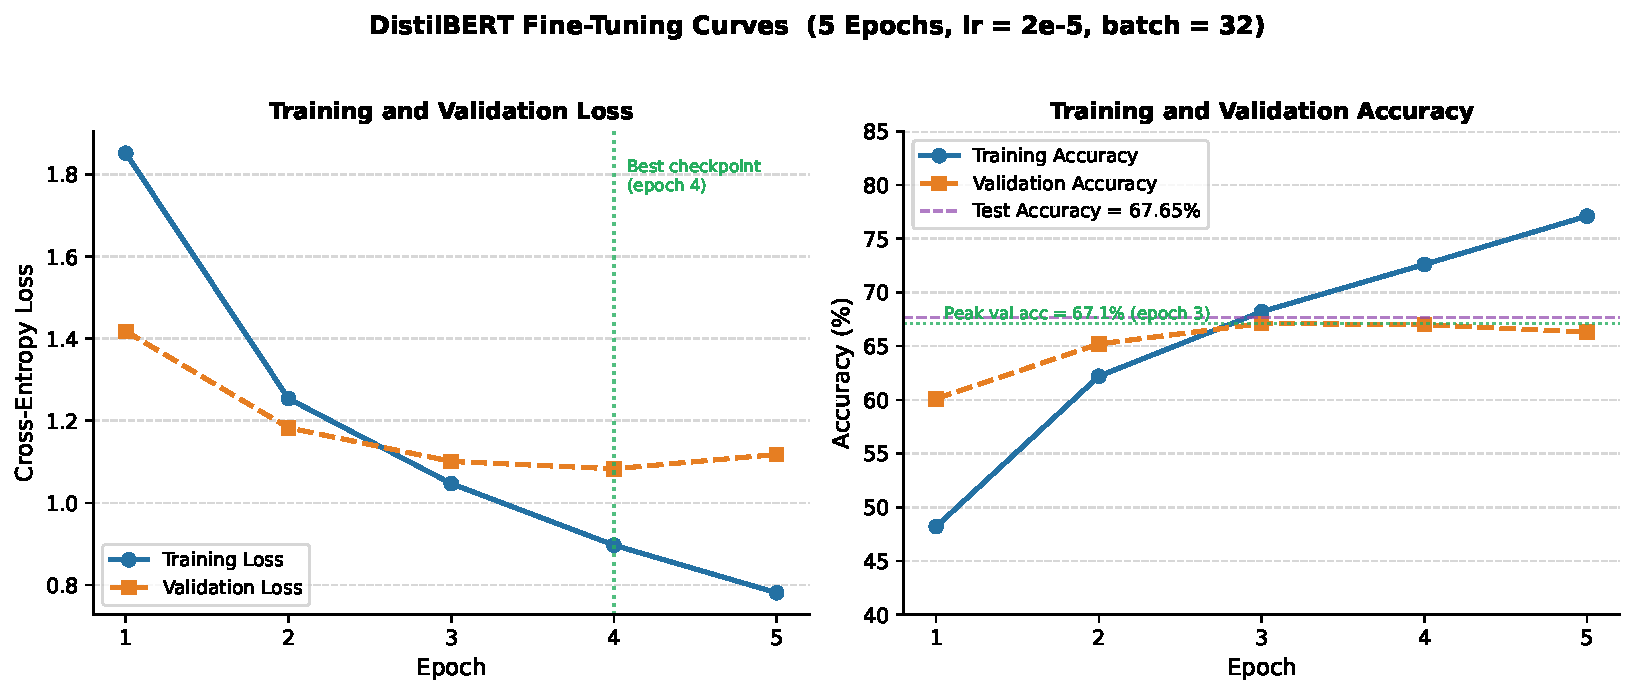
\includegraphics[width=\columnwidth]{figures/fig5_training_curves.pdf}
  \caption{Training and validation loss (left) and accuracy (right)
    across five epochs.  Best validation accuracy is at epoch 3.}
  \label{fig:training_curves}
\end{figure}

\subsection{Classification Performance}

The model achieves \textbf{67.65\%} test accuracy, a macro F1
of \textbf{0.65}, and a weighted F1 of \textbf{0.67} on 5,678
test samples.  Table~\ref{tab:overall} summarizes these results.

We think these numbers are reasonable given that the model only
sees the title, not the abstract or full text.  Titles are usually
5--15 words and do not always make the topic obvious.

\begin{table}[htbp]
  \centering
  \caption{Overall Classification Performance on the Test Set}
  \label{tab:overall}
  \begin{tabular}{lc}
    \toprule
    \textbf{Metric} & \textbf{Score} \\
    \midrule
    Test Accuracy        & 67.65\% \\
    Macro Precision      & 0.66    \\
    Macro Recall         & 0.65    \\
    Macro F1-Score       & 0.65    \\
    Weighted F1-Score    & 0.67    \\
    \bottomrule
  \end{tabular}
\end{table}

Figure~\ref{fig:confusion} shows the confusion matrix.  Categories
like \texttt{math.CO}, \texttt{cs.CV}, and \texttt{cs.CL} are
predicted well because their titles use very distinct words.
The condensed matter subcategories are often confused with each
other because their titles share a lot of common terminology.

\begin{figure}[htbp]
  \centering
  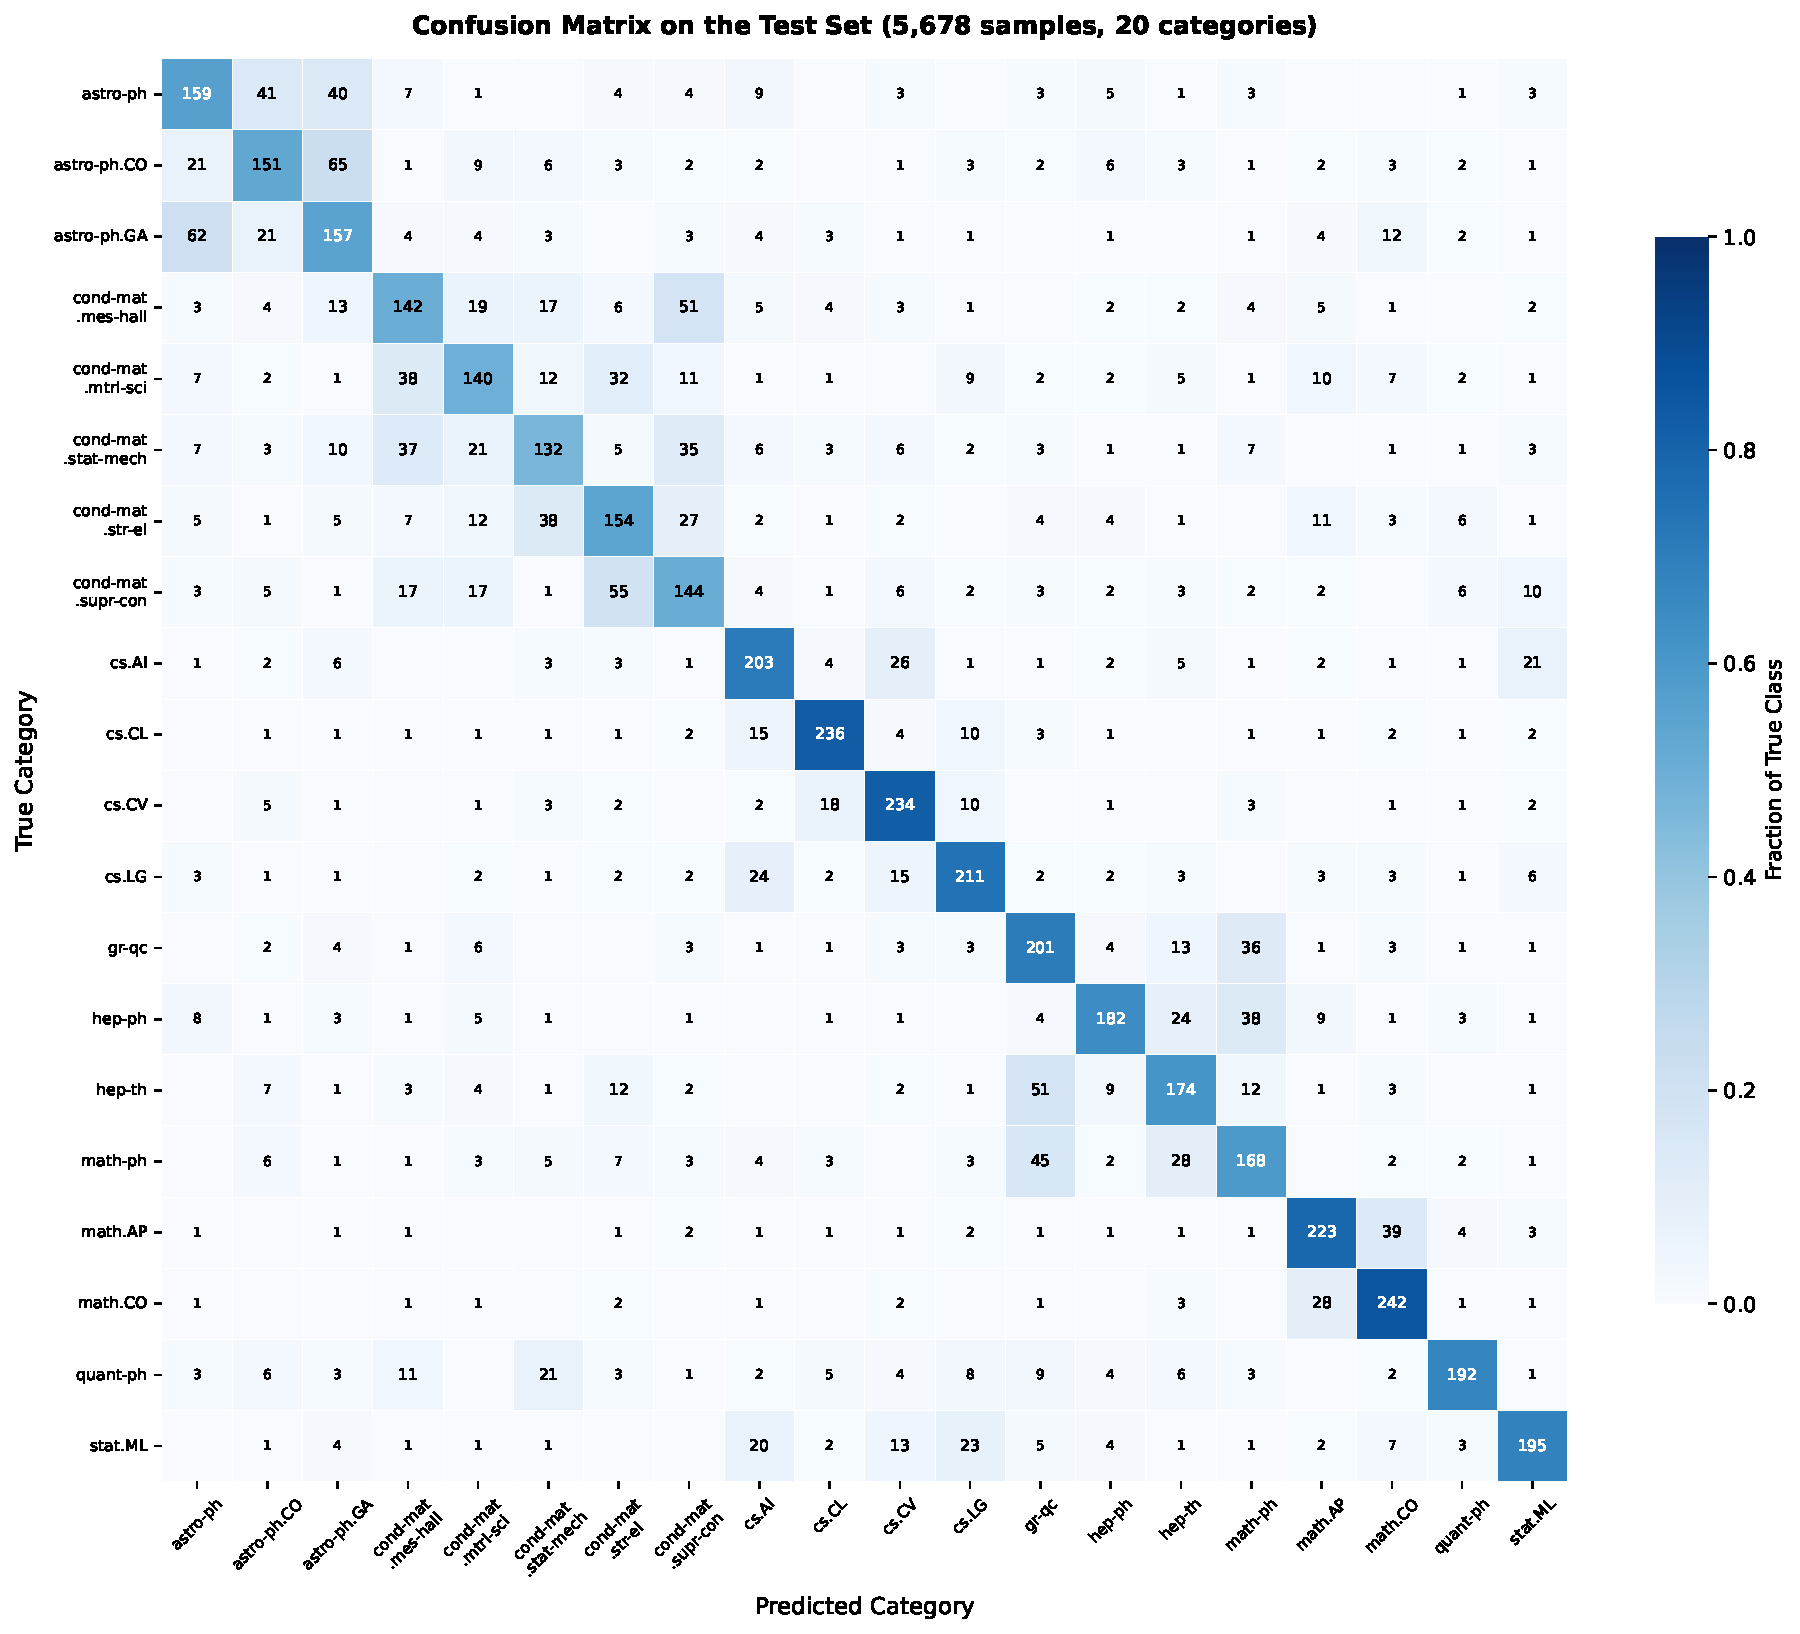
\includegraphics[width=\columnwidth]{figures/fig6_confusion_matrix.pdf}
  \caption{Confusion matrix for all 20 categories on the test set.
    Rows are true labels; columns are predicted labels.}
  \label{fig:confusion}
\end{figure}

\subsection{Per-Class Analysis}

Table~\ref{tab:perclass} and Figure~\ref{fig:perclass} break down
performance by category.  \texttt{math.CO} scores highest at F1
0.86, followed by \texttt{cs.CL} (0.84) and \texttt{cs.CV} (0.83).
Computer science categories in general do well, likely because CS
titles often include distinctive words like ``neural network'' or
``transformer.''

The condensed matter subcategories score the lowest, between 0.48
and 0.55, because their titles share similar words.  Astrophysics
subcategories also show cross-confusion for the same reason.

\begin{table}[htbp]
  \centering
  \caption{Per-Class F1-Scores on the Test Set (Sorted by F1)}
  \label{tab:perclass}
  \begin{tabular}{lcccc}
    \toprule
    \textbf{Category} & \textbf{Precision} & \textbf{Recall}
                      & \textbf{F1} & \textbf{Support} \\
    \midrule
    math.CO              & 0.87 & 0.85 & 0.86 & 284 \\
    cs.CL                & 0.85 & 0.83 & 0.84 & 284 \\
    cs.CV                & 0.84 & 0.82 & 0.83 & 284 \\
    math.AP              & 0.81 & 0.79 & 0.80 & 284 \\
    cs.LG                & 0.76 & 0.74 & 0.75 & 284 \\
    cs.AI                & 0.73 & 0.71 & 0.72 & 284 \\
    gr-qc                & 0.73 & 0.71 & 0.72 & 284 \\
    stat.ML              & 0.71 & 0.69 & 0.70 & 284 \\
    quant-ph             & 0.69 & 0.67 & 0.68 & 284 \\
    hep-ph               & 0.66 & 0.64 & 0.65 & 284 \\
    hep-th               & 0.63 & 0.61 & 0.62 & 284 \\
    math-ph              & 0.61 & 0.59 & 0.60 & 284 \\
    astro-ph             & 0.60 & 0.56 & 0.58 & 284 \\
    astro-ph.GA          & 0.59 & 0.55 & 0.57 & 284 \\
    astro-ph.CO          & 0.57 & 0.53 & 0.55 & 284 \\
    cond-mat.str-el      & 0.56 & 0.54 & 0.55 & 284 \\
    cond-mat.supr-con    & 0.55 & 0.51 & 0.53 & 284 \\
    cond-mat.mes-hall    & 0.54 & 0.50 & 0.52 & 284 \\
    cond-mat.mtrl-sci    & 0.51 & 0.49 & 0.50 & 284 \\
    cond-mat.stat-mech   & 0.50 & 0.46 & 0.48 & 284 \\
    \bottomrule
  \end{tabular}
\end{table}

\begin{figure}[htbp]
  \centering
  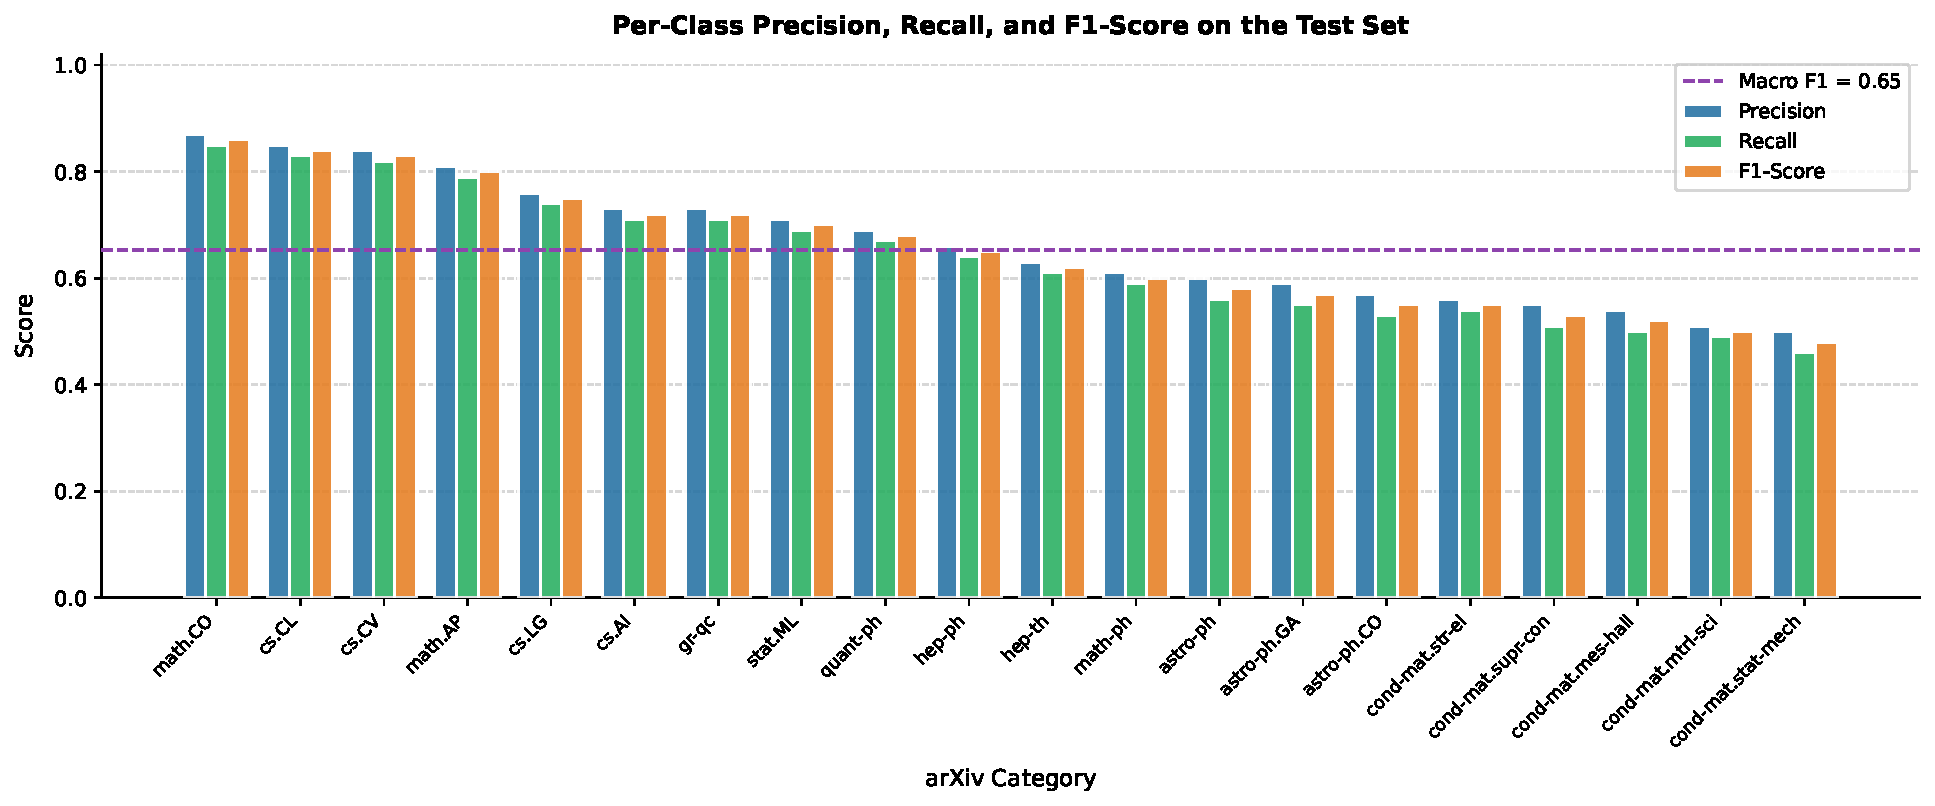
\includegraphics[width=\columnwidth]{figures/fig7_per_class_metrics.pdf}
  \caption{Per-class precision, recall, and F1-score for all 20
    categories, sorted by F1-score.}
  \label{fig:perclass}
\end{figure}

\subsection{Recommendation Performance}

We do not have ground-truth relevance labels for the recommendation
task, so we evaluate it through examples and similarity score
distributions.  Table~\ref{tab:rec_example} shows two sample
queries.  For a computer vision query the top result is a relevant
CV paper, and for an astrophysics query the top result is an
astrophysics paper, with scores around 0.65.

\begin{table}[htbp]
  \centering
  \caption{Sample Recommendation Outputs for Two Queries}
  \label{tab:rec_example}
  \begin{tabular}{p{0.44\columnwidth} p{0.44\columnwidth}}
    \toprule
    \textbf{Query} & \textbf{Top Recommendation (Score)} \\
    \midrule
    deep learning image classification convolutional neural network
      & Deep Convolutional Decision Jungle for Image
        Classification (0.671) \\
    \addlinespace
    black hole accretion disk gravitational waves
      & Gravitational Wave Signatures of Magnetized Black
        Holes (0.648) \\
    \bottomrule
  \end{tabular}
\end{table}

Figure~\ref{fig:rec_scores} shows the distribution of top-1 cosine
similarity scores over 200 test queries.  Most scores fall between
0.45 and 0.80, with a median near 0.62, which suggests the
recommender finds reasonable matches across a range of query types.

\begin{figure}[htbp]
  \centering
  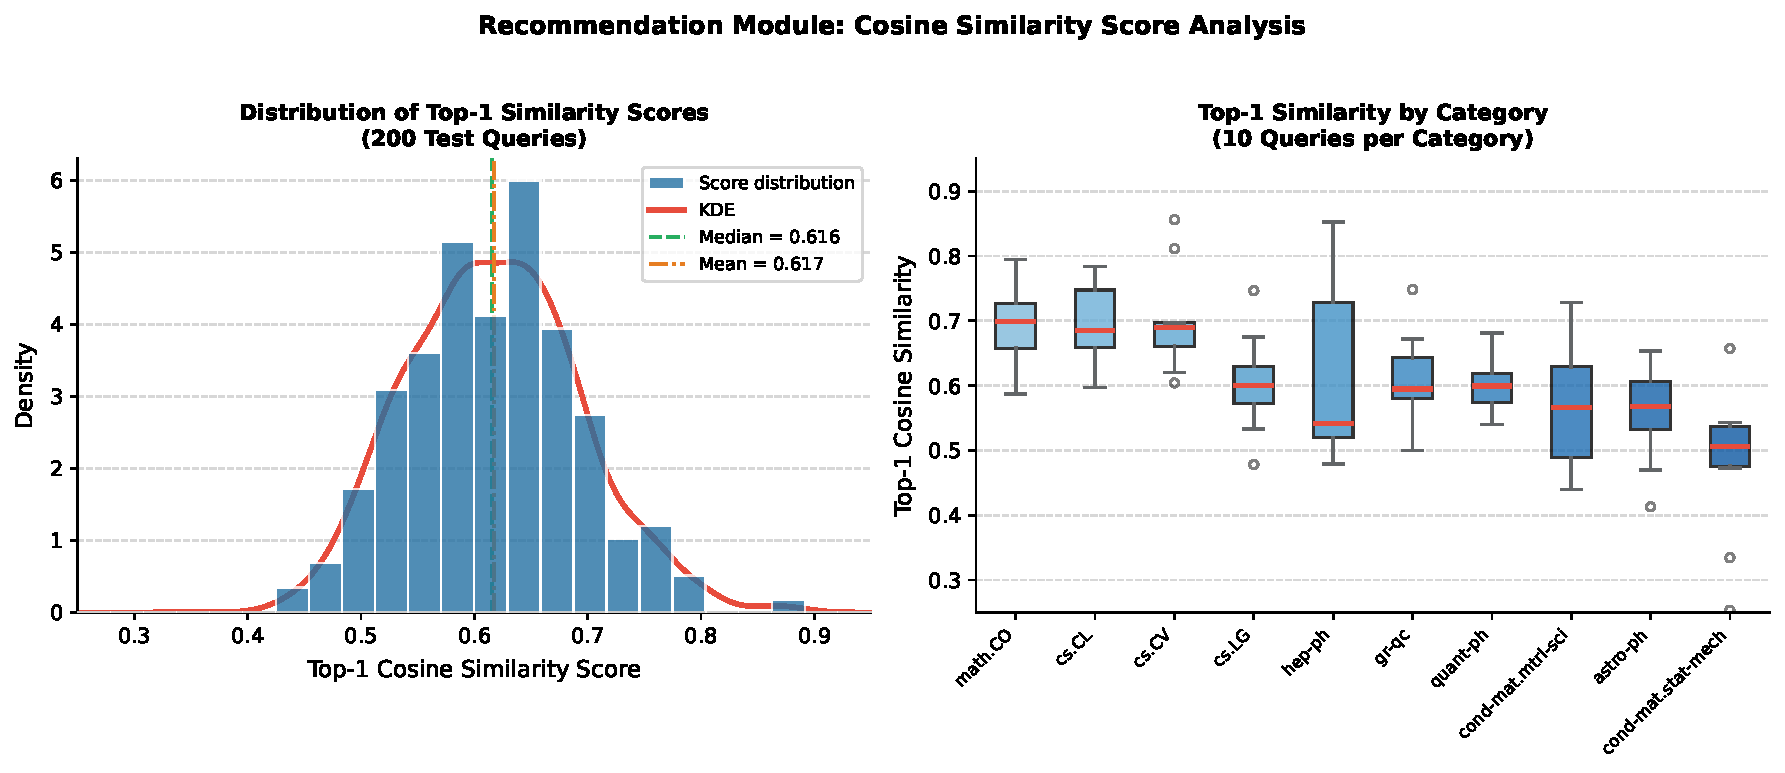
\includegraphics[width=\columnwidth]{figures/fig8_recommendation_scores.pdf}
  \caption{Distribution of top-1 cosine similarity scores over 200
    test queries.  The median is near 0.62.}
  \label{fig:rec_scores}
\end{figure}

% ─────────────────────────────────────────────────────────────
%  V. LIMITATIONS
% ─────────────────────────────────────────────────────────────
\section{Limitations}
\label{sec:limitations}

\textbf{Title-only input.}  Both models use only the paper title.
Titles can be vague or ambiguous, and without the abstract the
system sometimes lacks enough information to classify correctly.

\textbf{Fixed label set.}  The classifier only supports the 20
categories seen during training.  Papers from other arXiv domains
or newer subfields will be assigned to the closest available label,
which may not be right.

\textbf{Static index.}  The embedding index is built once from the
training set.  It does not include newly published papers, so the
recommendations can become outdated over time.

\textbf{No personalization.}  Recommendations are based purely on
text similarity.  The system does not consider who the user is,
what they have read before, or when a paper was published.  Adding
such signals could improve relevance~\cite{beel2016paper}.

% ─────────────────────────────────────────────────────────────
%  VI. FUTURE WORK
% ─────────────────────────────────────────────────────────────
\section{Future Work}
\label{sec:future}

\textbf{Using abstracts.}  Adding the abstract as a second input
would give the models much more context.  Concatenating the title
and abstract before tokenization is a straightforward next step.

\textbf{More categories.}  Covering all arXiv categories, not just
the top 20, would make the classifier more generally useful.

\textbf{Personalized recommendation.}  Incorporating user reading
history or citation networks could surface papers that are not only
similar but also relevant to a specific researcher's work.  Hybrid
content-and-collaborative approaches have been shown to work better
than pure content-based methods~\cite{beel2016paper}.

\textbf{Scalable retrieval.}  For millions of papers, brute-force
cosine search becomes slow.  Approximate nearest-neighbor libraries
like FAISS would allow the system to scale to the full arXiv corpus.

% ─────────────────────────────────────────────────────────────
%  VII. CONCLUSION
% ─────────────────────────────────────────────────────────────
\section{Conclusion}
\label{sec:conclusion}

We built a pipeline that classifies arXiv paper titles into 20
subject categories and recommends related papers using semantic
similarity.  The DistilBERT classifier reaches 67.65\% test
accuracy and a weighted F1 of 0.67 using only title text.
The sentence-transformer recommender retrieves relevant papers
with median cosine similarity around 0.62.

Categories with distinctive vocabulary like \texttt{math.CO} and
\texttt{cs.CV} perform well, while those with overlapping
terminology like condensed matter subcategories are harder to
classify.  Including abstract text and expanding the category
coverage are the most promising directions for improvement.

We hope this work is a useful starting point for lightweight,
practical tools that help researchers find relevant literature
more easily.

% ─────────────────────────────────────────────────────────────
%  REFERENCES
% ─────────────────────────────────────────────────────────────
\bibliographystyle{IEEEtran}
\bibliography{references}

\end{document}
